% ==========================================================
% ENTREGA 1 — O corpus do projeto
% Projeto Integrador III — Motor de Busca — Ciência de Dados
% Fatec Baixada Santista – Rubens Lara
% Grupo APPA
% ==========================================================

\documentclass[
  article,
  12pt,
  oneside,
  a4paper,
  english,
  brazil
]{abntex2}\usepackage[]{graphicx}\usepackage[]{xcolor}
% maxwidth is the original width if it is less than linewidth
% otherwise use linewidth (to make sure the graphics do not exceed the margin)
\makeatletter
\def\maxwidth{ %
  \ifdim\Gin@nat@width>\linewidth
    \linewidth
  \else
    \Gin@nat@width
  \fi
}
\makeatother

\definecolor{fgcolor}{rgb}{0.345, 0.345, 0.345}
\newcommand{\hlnum}[1]{\textcolor[rgb]{0.686,0.059,0.569}{#1}}%
\newcommand{\hlsng}[1]{\textcolor[rgb]{0.192,0.494,0.8}{#1}}%
\newcommand{\hlcom}[1]{\textcolor[rgb]{0.678,0.584,0.686}{\textit{#1}}}%
\newcommand{\hlopt}[1]{\textcolor[rgb]{0,0,0}{#1}}%
\newcommand{\hldef}[1]{\textcolor[rgb]{0.345,0.345,0.345}{#1}}%
\newcommand{\hlkwa}[1]{\textcolor[rgb]{0.161,0.373,0.58}{\textbf{#1}}}%
\newcommand{\hlkwb}[1]{\textcolor[rgb]{0.69,0.353,0.396}{#1}}%
\newcommand{\hlkwc}[1]{\textcolor[rgb]{0.333,0.667,0.333}{#1}}%
\newcommand{\hlkwd}[1]{\textcolor[rgb]{0.737,0.353,0.396}{\textbf{#1}}}%
\let\hlipl\hlkwb

\usepackage{framed}
\makeatletter
\newenvironment{kframe}{%
 \def\at@end@of@kframe{}%
 \ifinner\ifhmode%
  \def\at@end@of@kframe{\end{minipage}}%
  \begin{minipage}{\columnwidth}%
 \fi\fi%
 \def\FrameCommand##1{\hskip\@totalleftmargin \hskip-\fboxsep
 \colorbox{shadecolor}{##1}\hskip-\fboxsep
     % There is no \\@totalrightmargin, so:
     \hskip-\linewidth \hskip-\@totalleftmargin \hskip\columnwidth}%
 \MakeFramed {\advance\hsize-\width
   \@totalleftmargin\z@ \linewidth\hsize
   \@setminipage}}%
 {\par\unskip\endMakeFramed%
 \at@end@of@kframe}
\makeatother

\definecolor{shadecolor}{rgb}{.97, .97, .97}
\definecolor{messagecolor}{rgb}{0, 0, 0}
\definecolor{warningcolor}{rgb}{1, 0, 1}
\definecolor{errorcolor}{rgb}{1, 0, 0}
\newenvironment{knitrout}{}{} % an empty environment to be redefined in TeX

\usepackage{amsmath}
\usepackage{alltt}

\usepackage[T1]{fontenc}
\usepackage[utf8]{inputenc}
\usepackage{lmodern}
\usepackage{amsmath,amssymb}
\usepackage{icomma}
\usepackage{booktabs}
\usepackage{enumitem}
\usepackage{xcolor}
\usepackage[alf]{abntex2cite}

\setlist{noitemsep, topsep=3pt, parsep=1pt, partopsep=0pt}
\setlength{\parskip}{0.35em}

\hypersetup{hidelinks}

% ----------------------------------------------------------
% DADOS DA ENTREGA
% ----------------------------------------------------------
\titulo{O corpus do projeto: Clubes Tradicionais de Futebol da Baixada Santista}
\tituloestrangeiro{}
\autor{Grupo APPA}
\local{Santos-SP}
\data{\today}

\newcommand{\nomecurso}{Tecnologia em Ciência de Dados}
\newcommand{\nomedisciplina}{Projeto Integrador III --- Motor de Busca}
\newcommand{\nomeprofessor}{Prof.\ Dr.\ João Paulo Ferreira de Mello}
\newcommand{\repositorio}{https://github.com/kyl8/pi3}
\newcommand{\integrantes}{%
  Arthur Galvão \\
  Pedro Henrique \\
  Pedro Alvarenga \\
  Ailana%
}
\IfFileExists{upquote.sty}{\usepackage{upquote}}{}
\begin{document}





\selectlanguage{brazil}
\frenchspacing

% ----------------------------------------------------------
% IDENTIFICAÇÃO
% ----------------------------------------------------------
\maketitle

\begin{center}
  \small
  Fatec Baixada Santista -- Rubens Lara \\
  \nomecurso{} \quad|\quad \nomedisciplina{} \quad|\quad \nomeprofessor{} \\[0.3em]
  \integrantes \\[0.3em]
  Repositório: \texttt{\repositorio}
\end{center}



\textual

% ==========================================================================
\section{Introdução}
% ==========================================================================

O presente projeto tem como tema a recuperação de informação histórica e patrimonial dos três clubes centenários de futebol da Baixada Santista: Santos Futebol Clube, Associação Atlética Portuguesa e Jabaquara Atlético Clube. A região de Santos possui uma das trajetórias futebolísticas mais expressivas do Brasil, abrigando agremiações pioneiras que participaram ativamente da estruturação do esporte paulista no início do século XX e influenciaram a cultura litorânea.

O motor de busca proposto destina-se a pesquisadores de história esportiva, estudantes de ciência de dados, jornalistas e torcedores que buscam consultar dados objetivos sobre a memória esportiva regional. Em recuperação de informação, a modelagem busca satisfazer a necessidade de informação do usuário de forma precisa, sem exigir que a pessoa conheça antecipadamente a terminologia técnica exata da base \cite[cap.~1]{manning2008}. Com base nesse princípio, o sistema foi concebido para atender a três necessidades centrais:
\begin{enumerate}
  \item \textbf{Fundação, origens e cores:} identificar a data e o contexto histórico de fundação dos clubes, assim como suas cores e símbolos representativos;
  \item \textbf{Estádios e patrimônio físico:} localizar dados sobre os estádios das equipes (Vila Belmiro, Ulrico Mursa e Caneleira) e sua infraestrutura patrimonial;
  \item \textbf{Títulos e rivalidades regionais:} consultar conquistas marcantes, rivalidades históricas e confrontos locais, a exemplo do Clássico das Praias.
\end{enumerate}

Este relatório formaliza a Entrega 1 do projeto: documenta a fonte e a licença dos dados, detalha as etapas de coleta automatizada, reporta as dificuldades operacionais encontradas e apresenta a defesa empírica da suficiência do corpus coletado.

% ==========================================================================
\section{A fonte e o documento}
% ==========================================================================

O corpus foi obtido a partir da Wikipédia em língua portuguesa \cite{wikipedia}, sob licença livre Creative Commons Atribuição-CompartilhaIgual 4.0 Internacional (CC BY-SA 4.0), com coleta efetuada em 2026. Foram extraídas três páginas principais: \texttt{Santos Futebol Clube}, \texttt{Associação Atlética Portuguesa (Santos)} e \texttt{Jabaquara Atlético Clube}. No total, o acervo consolidado reúne $N = \text{141}$ documentos extraídos de $\text{3}$ páginas enciclopédicas.

A unidade de documento adotada é o \emph{parágrafo textual} ($<\!\text{p}\!>$). A escolha do parágrafo fundamenta-se na granularidade de recuperação: adotar o artigo enciclopédico inteiro como um único documento implicaria que uma busca sobre a capacidade da Vila Belmiro retornaria a página completa de dezenas de páginas do Santos FC, exigindo navegação manual exaustiva do usuário. Por outro lado, a segmentação por frases isoladas produziria fragmentos com contexto semântico insuficiente. O parágrafo enciclopédico configura, portanto, a menor unidade autossuficiente capaz de responder integralmente a uma consulta específica.

A adoção da Wikipédia como fonte deve-se à qualidade da redação colaborativa, à perenidade dos fatos históricos relatados e à acessibilidade de sua estrutura textual. Como alternativa, avaliou-se inicialmente a extração a partir de sites institucionais oficiais e páginas de torcidas organizadas. Essa opção foi descartada por apresentar formatações instáveis, conteúdo promocional de vendas de ingressos e ausência de licença aberta uniforme para reuso de dados.

% ==========================================================================
\section{Como o corpus foi obtido}
% ==========================================================================

A coleta foi estruturada em script computacional reprodutível em linguagem R, registrado no repositório. O fluxo operou em cinco etapas sequenciais:
\begin{enumerate}
  \item \textbf{Requisição e parsing:} obtenção do código HTML das três páginas selecionadas na Wikipédia;
  \item \textbf{Isolamento de parágrafos:} seleção dos nós $<\!\text{p}\!>$ pertencentes ao corpo principal da página enciclopédica;
  \item \textbf{Sanitização textual:} remoção de tags de hyperlink, eliminação sistemática de notas sobrescritas de rodapé (como \texttt{[1]} ou \texttt{[nota 2]}) e expurgo de caracteres residuais de escape;
  \item \textbf{Filtragem por tamanho mínimo:} aplicação do limiar de corte de \text{50} caracteres, eliminando legendas órfãs, linhas de navegação e parágrafos sem densidade informativa;
  \item \textbf{Serialização:} salvamento dos vetores nomeados de documentos e procedência nos arquivos \texttt{docs.rds} e \texttt{origem.rds}.
\end{enumerate}

Durante o processo de extração, três desafios operacionais foram contornados:
\begin{itemize}
  \item \textbf{Desambiguação de títulos:} a busca inicial por ``Portuguesa'' remetia à Associação Portuguesa de Desportos (da capital paulista); foi necessário fixar explicitamente o título \texttt{Associação Atlética Portuguesa (Santos)};
  \item \textbf{Fragmentos residuais:} elementos pertencentes a caixas de navegação lateral (\emph{infoboxes}) foram inicialmente capturados como parágrafos curtos, sendo sanados pelo refinamento do seletor CSS restrito ao corpo textual principal;
  \item \textbf{Disparidade no volume de texto:} a projeção internacional do Santos FC resulta em um artigo substancialmente mais longo do que os dos clubes coirmãos, questão gerenciada na defesa técnica a seguir.
\end{itemize}

% ==========================================================================
\section{Defesa do corpus}
% ==========================================================================

A Tabela~\ref{tab:diag} sumariza o diagnóstico técnico do corpus, acompanhada pela Tabela~\ref{tab:origem} com a distribuição dos documentos por página.

\begin{table}[!htbp]
  \centering
  \begin{minipage}[t]{0.53\textwidth}
    \caption{Diagnóstico do corpus}
    \label{tab:diag}
    \scriptsize
    \begin{tabular}{@{}p{0.36\textwidth}p{0.60\textwidth}@{}}
      \toprule
      \textbf{Verificação} & \textbf{Resultado} \\
      \midrule
      Tamanho & $\text{141}$ docs de $\text{3}$ págs. \\
      Tokens/doc & 8 a 322 (m\'edia 83,6) \\
      Vocabulário & $\text{2517}$ termos ($\text{11794}$ tokens) \\
      Domínio & \texttt{Santos FC}: 107 de 141 (76\%) \\
      Suspeitos & 7 com menos de 20 tokens; 2 com mais de 300 \\
      Sujeira & 141 com acento, 141 com pontua\c{c}\~ao, 135 com d\'igitos (de 141) \\
      \bottomrule
    \end{tabular}
    \fonte{Elaborada pelos autores.}
  \end{minipage}\hfill
  \begin{minipage}[t]{0.43\textwidth}
    \caption{Documentos por página}
    \label{tab:origem}
    \scriptsize

\begin{tabular}{lrr}
\toprule
P\'agina & Documentos & Tokens (m\'edia)\\
\midrule
Santos FC & 107 & 91,7\\
Portuguesa Santista & 23 & 53,3\\
Jabaquara & 11 & 68,8\\
\bottomrule
\end{tabular}


    \fonte{Elaborada pelos autores.}
  \end{minipage}
\end{table}

\textbf{Tamanho.} O corpus conta com $\text{141}$ documentos, superando a faixa de referência (20 a 60). Essa densidade garante suporte estatístico aos cálculos de matriz termo-documento e IDF das próximas etapas.

\textbf{Domínio de página.} A Tabela~\ref{tab:origem} evidencia o predomínio do Santos FC (\texttt{Santos FC}: 107 de 141 (76\%)), reflexo natural do acervo disponível. A presença de 34 documentos dos demais clubes assegura que o motor recupere dados sobre a história regional integrada.

\textbf{Comprimento e distribuição.} A Figura~\ref{fig:tam} exibe o perfil unimodal de tokens por parágrafo (média de \text{83,6}), confirmando regularidade estrutural.

\begin{figure}[!htbp]
  \centering
  \caption{Distribuição de tokens por documento}
  \label{fig:tam}
\begin{knitrout}
\definecolor{shadecolor}{rgb}{0.969, 0.969, 0.969}\color{fgcolor}

{\centering 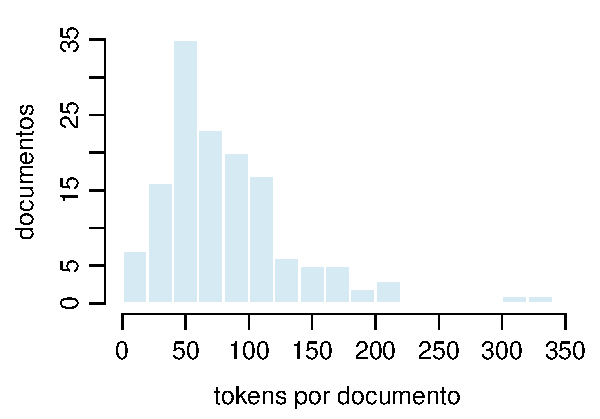
\includegraphics[width=0.48\linewidth]{figure/fig-tam-1} 

}


\end{knitrout}
  \fonte{Elaborada pelos autores.}
\end{figure}

\textbf{Sujeira e vocabulário.} Os dez termos mais frequentes são \texttt{o}, \texttt{de}, \texttt{a}, \texttt{e}, \texttt{em}, \texttt{do}, \texttt{santos}, \texttt{da}, \texttt{no}, \texttt{na}, sendo \texttt{santos} o único termo temático no topo. Os demais são palavras gramaticais (\emph{stopwords}), comprovando a necessidade do pré-processamento da Aula 03.

\textbf{Veredito.} O corpus atende plenamente às três necessidades de informação e está pronto e serializado para as etapas subsequentes.

% ----------------------------------------------------------
% REFERÊNCIAS
% ----------------------------------------------------------
\postextual
\bibliography{referencias}

\end{document}
